%%%%%%%%%%%%%%%%%%%%%%%%%%%%%%%%%%%%%%%%%%%%%%%%%%%%%%%%%%%%%%%%%%%%%%%%%%%%%%%%
% \section{Discussion of Polarized Sea Asymmetry}
%%%%%%%%%%%%%%%%%%%%%%%%%%%%%%%%%%%%%%%%%%%%%%%%%%%%%%%%%%%%%%%%%%%%%%%%%%%%%%%%

In this section, we take the distributions from the previous section after all corrections, shown in Fig.~\ref{fig:helicity-transversity}, and discuss
the physics implications. We will focus on the results new to this paper, mainly the
isovector helicity and nucleon transversity distribution. 
We strongly believe that it is worth more lattice-QCD effort to improve our knowledge of the polarized
PDFs, which still lack precision experimental data over most $x$ regions, especially
the antiquark distribution, which we emphasize in this section. 

%%%%%%%%%%%%%%%%%%%%%%%%%%%%%%%%%%%%%%%%
% Helicity
The left panel of Fig.~\ref{fig:helicity-transversity} shows the helicity distribution
$x (\Delta u(x)-\Delta d(x))$, along with selected recent global analyses
by JAM~\cite{Jimenez-Delgado:2013boa}, CCVS09~\cite{deFlorian:2009vb}, and
NNPDFpol1.1~\cite{Nocera:2014gqa}, whose nucleon isovector distribution uncertainties have been ignored.
Also note that the plots now show the distribution multiplied by $x$,
since this form is used in global-analysis parametrizations.
%We see more weight distributed near the large-$x$ region, which could shift as we lower the light-quark masses or increase the $P_z$ value in the calculation.
We see more weight distributed in the large-$x$ region, which could shift toward smaller $x$ as we lower 
the quark masses. This is because lower quark mass increases the long-range correlations in ${\Delta h}_\text{lat}(z)$,
which in turn increases the small-$x$ contribution in the Fourier transformation. 
Since the increasing small-$x$ distribution will decrease the large-$x$ distribution due to charge conservation,
we expect this inconsistency to reduce as we go to smaller quark mass. 
%
We see there are noticeable differences between the extracted polarized PDFs
depending on the experimental cuts, theory inputs, parametrization, and so on.
For example, JAM excludes SIDIS data, leaving the sign of the light antiquark
determined by the valence and the magnitude determined from sum rules. 
DSSV also relies on assumptions such as SU(3) symmetry to constrain the 
analysis and adds a very small symmetry-breaking term. A direct lattice study
of hyperon axial couplings~\cite{Lin:2007ap} suggested that SU(3) breaking is
roughly 20\% at the physical point, bigger than these assumptions. 
Similar assumptions also made in the NNPDFpol1.1~\cite{Nocera:2014gqa}.
These assumptions are unavoidable due to the difficulties of getting constraint data from polarized experiments.
%
Future experiments with neutral- and
charged-current DIS (such as at EIC) will provide useful measurements
to constrain our understanding of the antiquark helicity distribution.

Our result for antiquark helicity favor more polarized up quark than down
flavor\footnote{Note that one should ignore the $x\in\{-0.08,0.08\}$ regions
since there is large uncertainty associated with the distribution in this region.},
which is consistent with the current PDF analysis and model
calculations, such as chiral quark soliton model
($\chi$QSM)~\cite{Schweitzer:2001sr}. This was first pointed out in
our earlier paper~\cite{Lin:2014zya} (using a different mass-correction formulation), which concentrated on
the sea flavor asymmetry in the unpolarized distribution; it was also noted in
preliminary studies in conference proceedings~\cite{Lin:2014gaa,Lin:2014yra,Lin:2015vxw}. The sea flavor asymmetry was
confirmed in the full analysis of the Run-9 data by both
STAR~\cite{Adamczyk:2014xyw} and PHENIX~\cite{Adare:2015gsd} collaborations.
RHIC experiments on longitudinal single-spin asymmetry and
parity-violating $W$ production at RHIC might shed more light on the
polarized sea distribution~\cite{Aschenauer:2013woa}.

We see a moderate polarized total sea asymmetry,
$\int_{0.08}^1 \Delta \overline{u}(x)-\Delta \overline{d}(x)=0.14(9)$, which is smaller than the previous determination~\cite{Lin:2014zya} but still consistent within errors. The update is due to the application of the mass-correction formula of Eq.~\ref{h_mass} instead of Eq.~\ref{Knbar}. The latter requires transforming back and forth between the PDF and moments, which introduces oscillatory artifacts.
Most QCD models predict smaller polarized sea asymmetry;
for example, see the recent review article by Chang and Peng,
in particular Table~5 of Ref.~\cite{Chang:2014jba}. 
$\chi$QSM, a large-$N_c$ model,
gives rather different results by predicting a large polarized sea asymmetry: 0.31.
Unfortunately, our current statistical error does not   
help rule out many models yet based on the total sea asymmetry.
On the experimental global analysis side, the total polarized sea asymmetry estimated by DSSV09 is
consistent with zero within 2 sigma, and the central value is also smaller ($\approx 0.07$)
than the unpolarized case. Current results for STAR~\cite{Adamczyk:2014xyw}
and PHENIX~\cite{Adare:2015gsd} in the middle-$x$ range do not clarify what the total
asymmetry would be.
The upcoming RHIC data from Run-13 with significantly improved statistics may
shed some light on this matter.
The upcoming Fermilab Drell-Yan experiments (E1027/E1039) can also provide precise
experimental input on the polarized sea asymmetry magnitude.

%%%%%%%%%%%%%%%%%%%%%%%%%%%%%%%%%%%%%%%%
% Transversity
The transversity distribution is the least known PDF among the three
PDF structures studied;
there is much less information available due to the difficulties in experiments.
There have been a few attempts to extract the transversity distribution, but
they suffer from fundamental defects.
Ref.~\cite{Anselmino:2008jk} makes various assumptions such as the evolution form and that there is no antiquark contribution.
Ref.~\cite{Radici:2013vra} uses dihadron fragmentation functions using data from HERMES and COMPASS analysis of pion-pair production in DIS off a transversely polarized target for two combinations of ``valence'' ($q+\bar{q}$)
helicity distribution. They have a proper $Q^2$ evolution but still rely on
assumptions such as the Soffer inequality.
Kang et~al.~\cite{Kang:2015msa} has improved evolutions implemented in their analysis, but they also make the assumption
that the sea asymmetry is zero. The distribution for the positive $x$ goes quickly to zero,
likely due to lack of data.

Our transversity result is shown in the
the right panel of Fig.~\ref{fig:helicity-transversity}, along with an estimate from a QCD model,
$\chi$QSM~\cite{Schweitzer:2001sr} and the latest transversity fit from Ref.~\cite{Kang:2015msa}\footnote{Note that the error band of this isovector structure from Kang et~al. has been added up linearly from the up and down components due to the asymmetric errorband reported in the components; the error given here might be larger than if derived using the correlations of the original analysis. Also, note that the scale is set at $10\mbox{ GeV}^2$; however, there is only a small difference in their central values between lower-$Q^2$ scale and $10\mbox{ GeV}^2$.}.
Surprisingly, our result is rather similar to $\chi$QSM within 90\% confidence, but with slower descent to zero in 
the $x\approx 1$ region, similar to the quark distribution. This can be, again, due to the heavier pion mass used in the 
calculation, as well as the need to push for even larger momenta.
In contrast, the phenomenological results from Ref.~\cite{Kang:2015msa} fall faster as $x$ approaches near 1.

Our result favors $\delta \overline{d}(x) > \delta \overline{u}(x)$ with total sea asymmetry
0.10(8), whose central value is still larger than most model predictions (for example, $\chi$QSM estimates $0.082$ asymmetry)
and in contradiction to the assumption that the antiquark is consistent with zero in some
transversity extractions using experimental data~\cite{Anselmino:2008jk,Radici:2013vra,Kang:2014zza,Kang:2015msa}. 
One interesting thing to note is that the central values of the lattice determination of the tensor charge $g_T$ (that is, $\int_{-1}^{+1} \delta u(x) -\delta d(x)$) extrapolated to the continuum limit from various groups are consistently higher than the phenomenological ones who assume zero total sea asymmetry in transversity; see the summary plot Fig.~10 in Ref.~\cite{Bhattacharya:2015wna}. This may indicate nonzero sea contribution with the same sign as our prediction here, or missing larger-$x$ data in containing their fit. 
It would be interesting to see whether such a nonzero sea asymmetry remains in the future high-statistics physical quark mass ensemble; it is certainly contrary to traditional expectation. Improved phenomenological analysis with new experimental data would also help to narrow the phenomenological uncertainties and explore the discrepancy.

The cleanest measurement of the transversity would have both a polarized beam and polarized target, but given the limited setups available, once again, more data are needed.
PHENIX and STAR will be able to help give more insight into this quantity.
Planned experiments, such as SoLID at Jefferson Lab, can provide good transversity measurements for a wide range of positive $x$.
The Drell-Yan experiment at FNAL (E1027+E1039) can in principle extract
sea-asymmetry information in the near future to settle the size of the total transversely polarized sea.

%%%%%%%%%%%%%%%%%%%%%%%%%%%%%%%%%%%%%%%%%%%%%%%%%%%%%%%%%%%%%%%%%%%%%%%%%%%%%%%%
\section*{Acknowledgments}
%%%%%%%%%%%%%%%%%%%%%%%%%%%%%%%%%%%%%%%%%%%%%%%%%%%%%%%%%%%%%%%%%%%%%%%%%%%%%%%%

The LQCD calculations were performed using the Chroma software
suite~\cite{Edwards:2004sx}.
Computations for this work were carried out in part on facilities of the
USQCD Collaboration, which are funded by the Office of Science of the
U.S. Department of Energy, and on Hyak clusters at the University of Washington
managed by UW Information Technology, using hardware awarded by NSF grant
PHY-09227700.
We thank MILC Collaboration for sharing the lattices used to perform this study.
%
This work was partially supported by the U.S. Department of Energy via grants DE-FG02-93ER-40762, a grant (No.~11DZ2260700) from the Office of Science and Technology in Shanghai Municipal Government, grants from National Science Foundation of China (No.~11175114, No.~11405104), a DFG grant SCHA~458/20-1, the Ministry of Science and Technology, Taiwan under Grant Nos.~102-2112-M-002-013-MY3 and 105-2918-I-002 -003 and the CASTS of NTU. The work of HWL and SDC were supported by the DOE grant DE-FG02-97ER4014 and DE-FG02-00ER41132.
The work of HWL is currently supported in part by the M. Hildred Blewett Fellowship of the American Physical Society, www.aps.org.
%
HWL thanks the Institute for Nuclear Theory at the University of Washington for its hospitality during the completion of this work. JWC would like to thank the hospitality of the Rudolph Peierls Centre for Theoretical Physics of the University of Oxford and Oxford Holography group, DAMTP of University of Cambridge, and 
Helmholtz-Institut f\"{u}r Strahlen- und Kernphysik and Bethe Center for Theoretical Physics, Universit\"{a}t Bonn.

\begin{figure*}
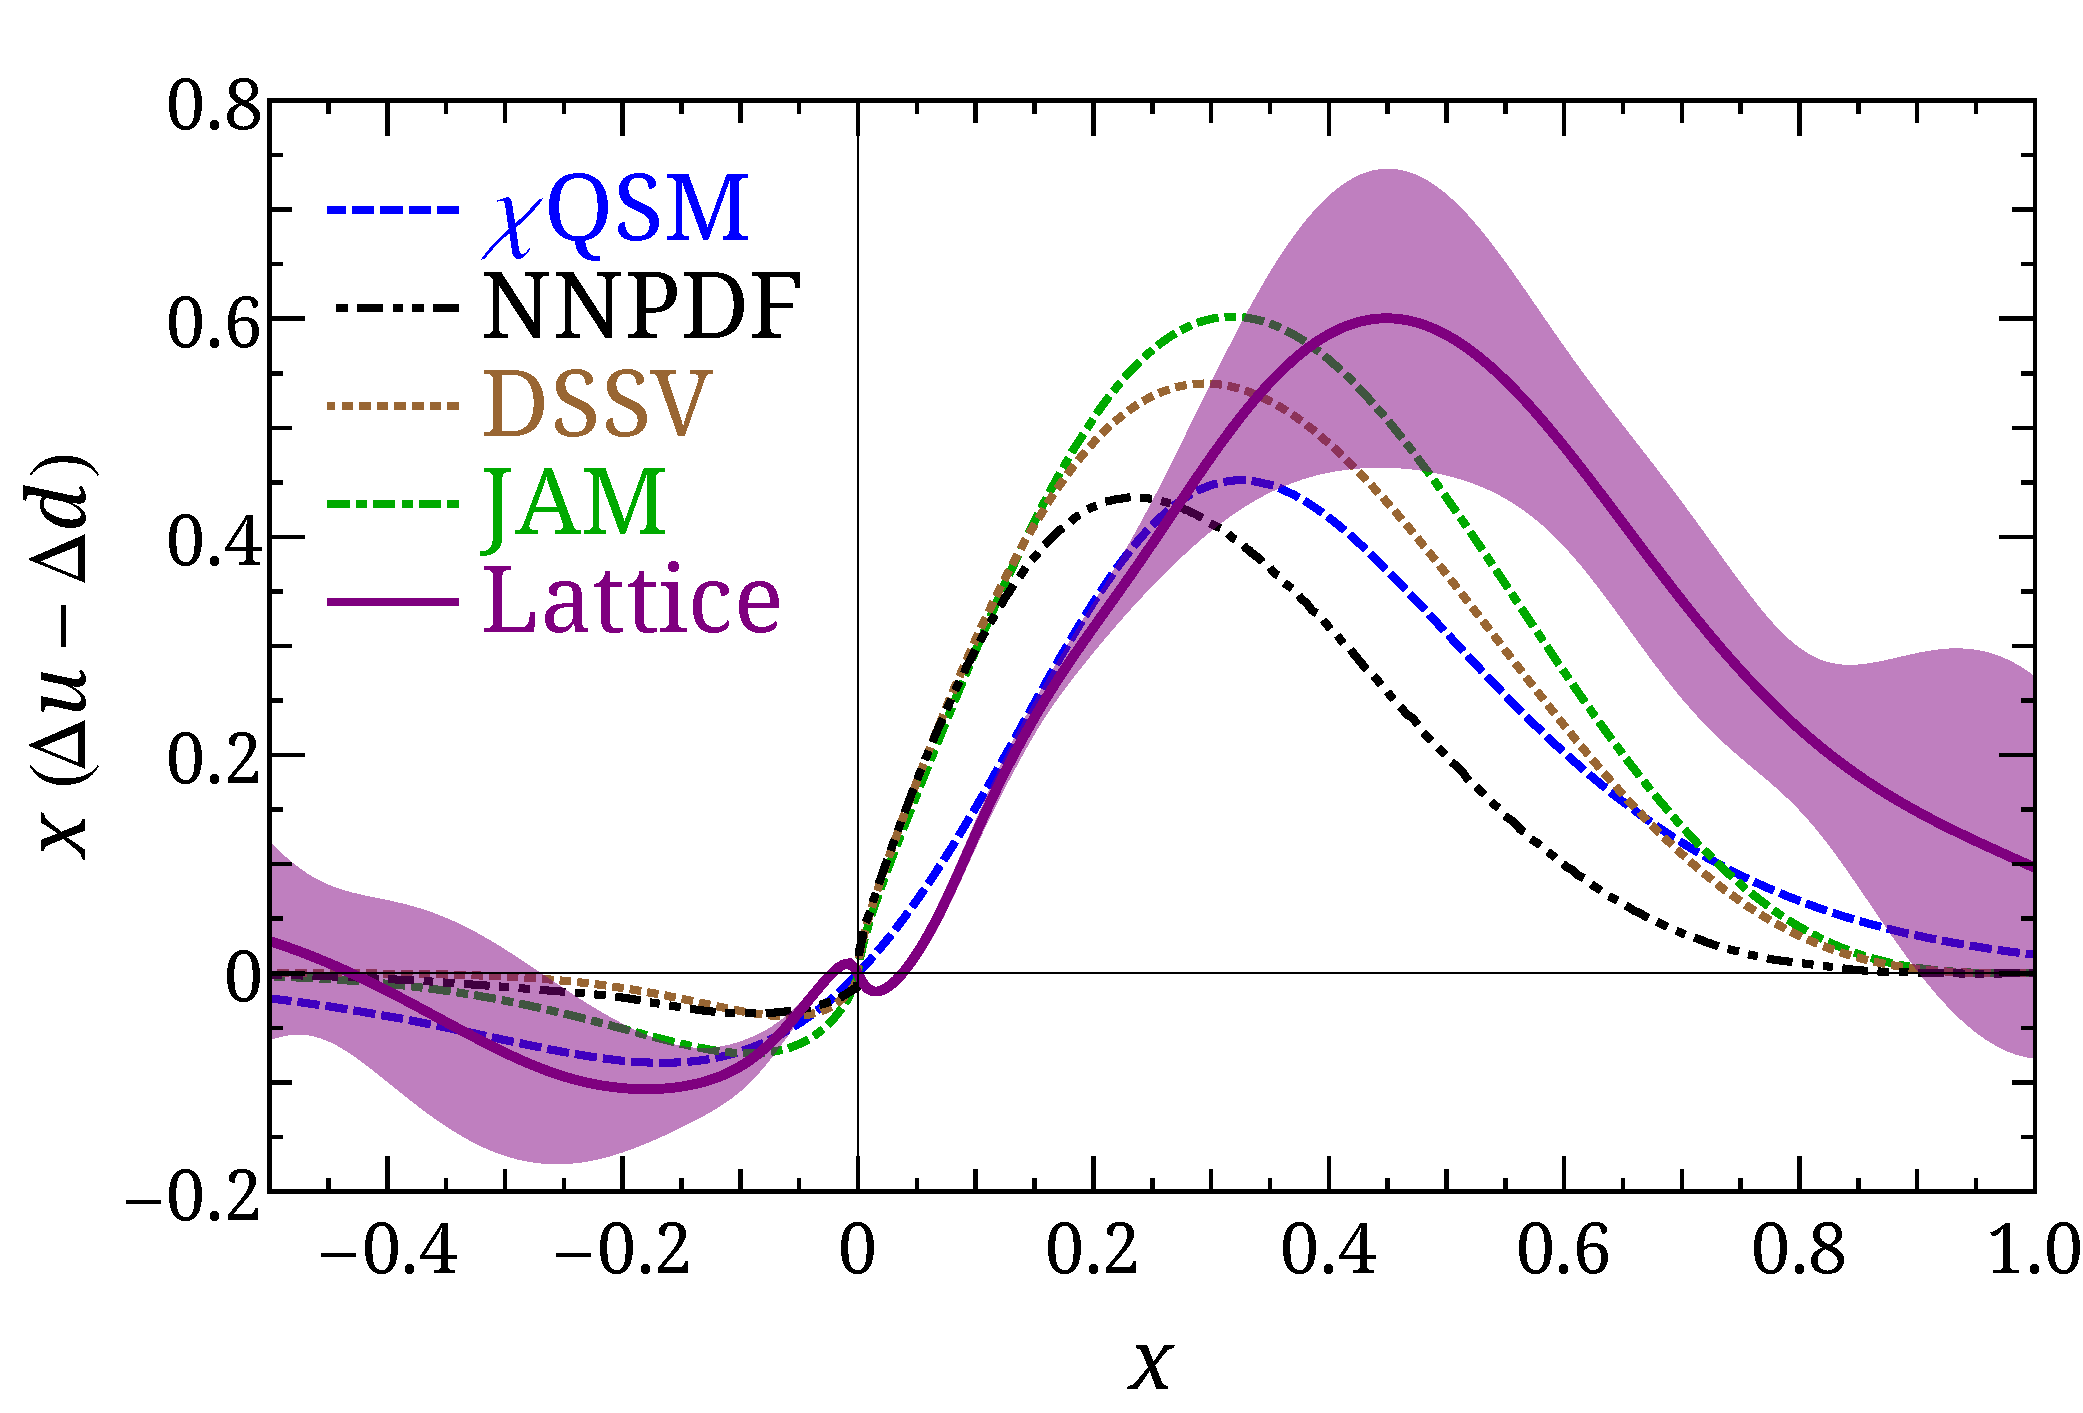
\includegraphics[width=0.47\textwidth]{images/helicityxfinal}
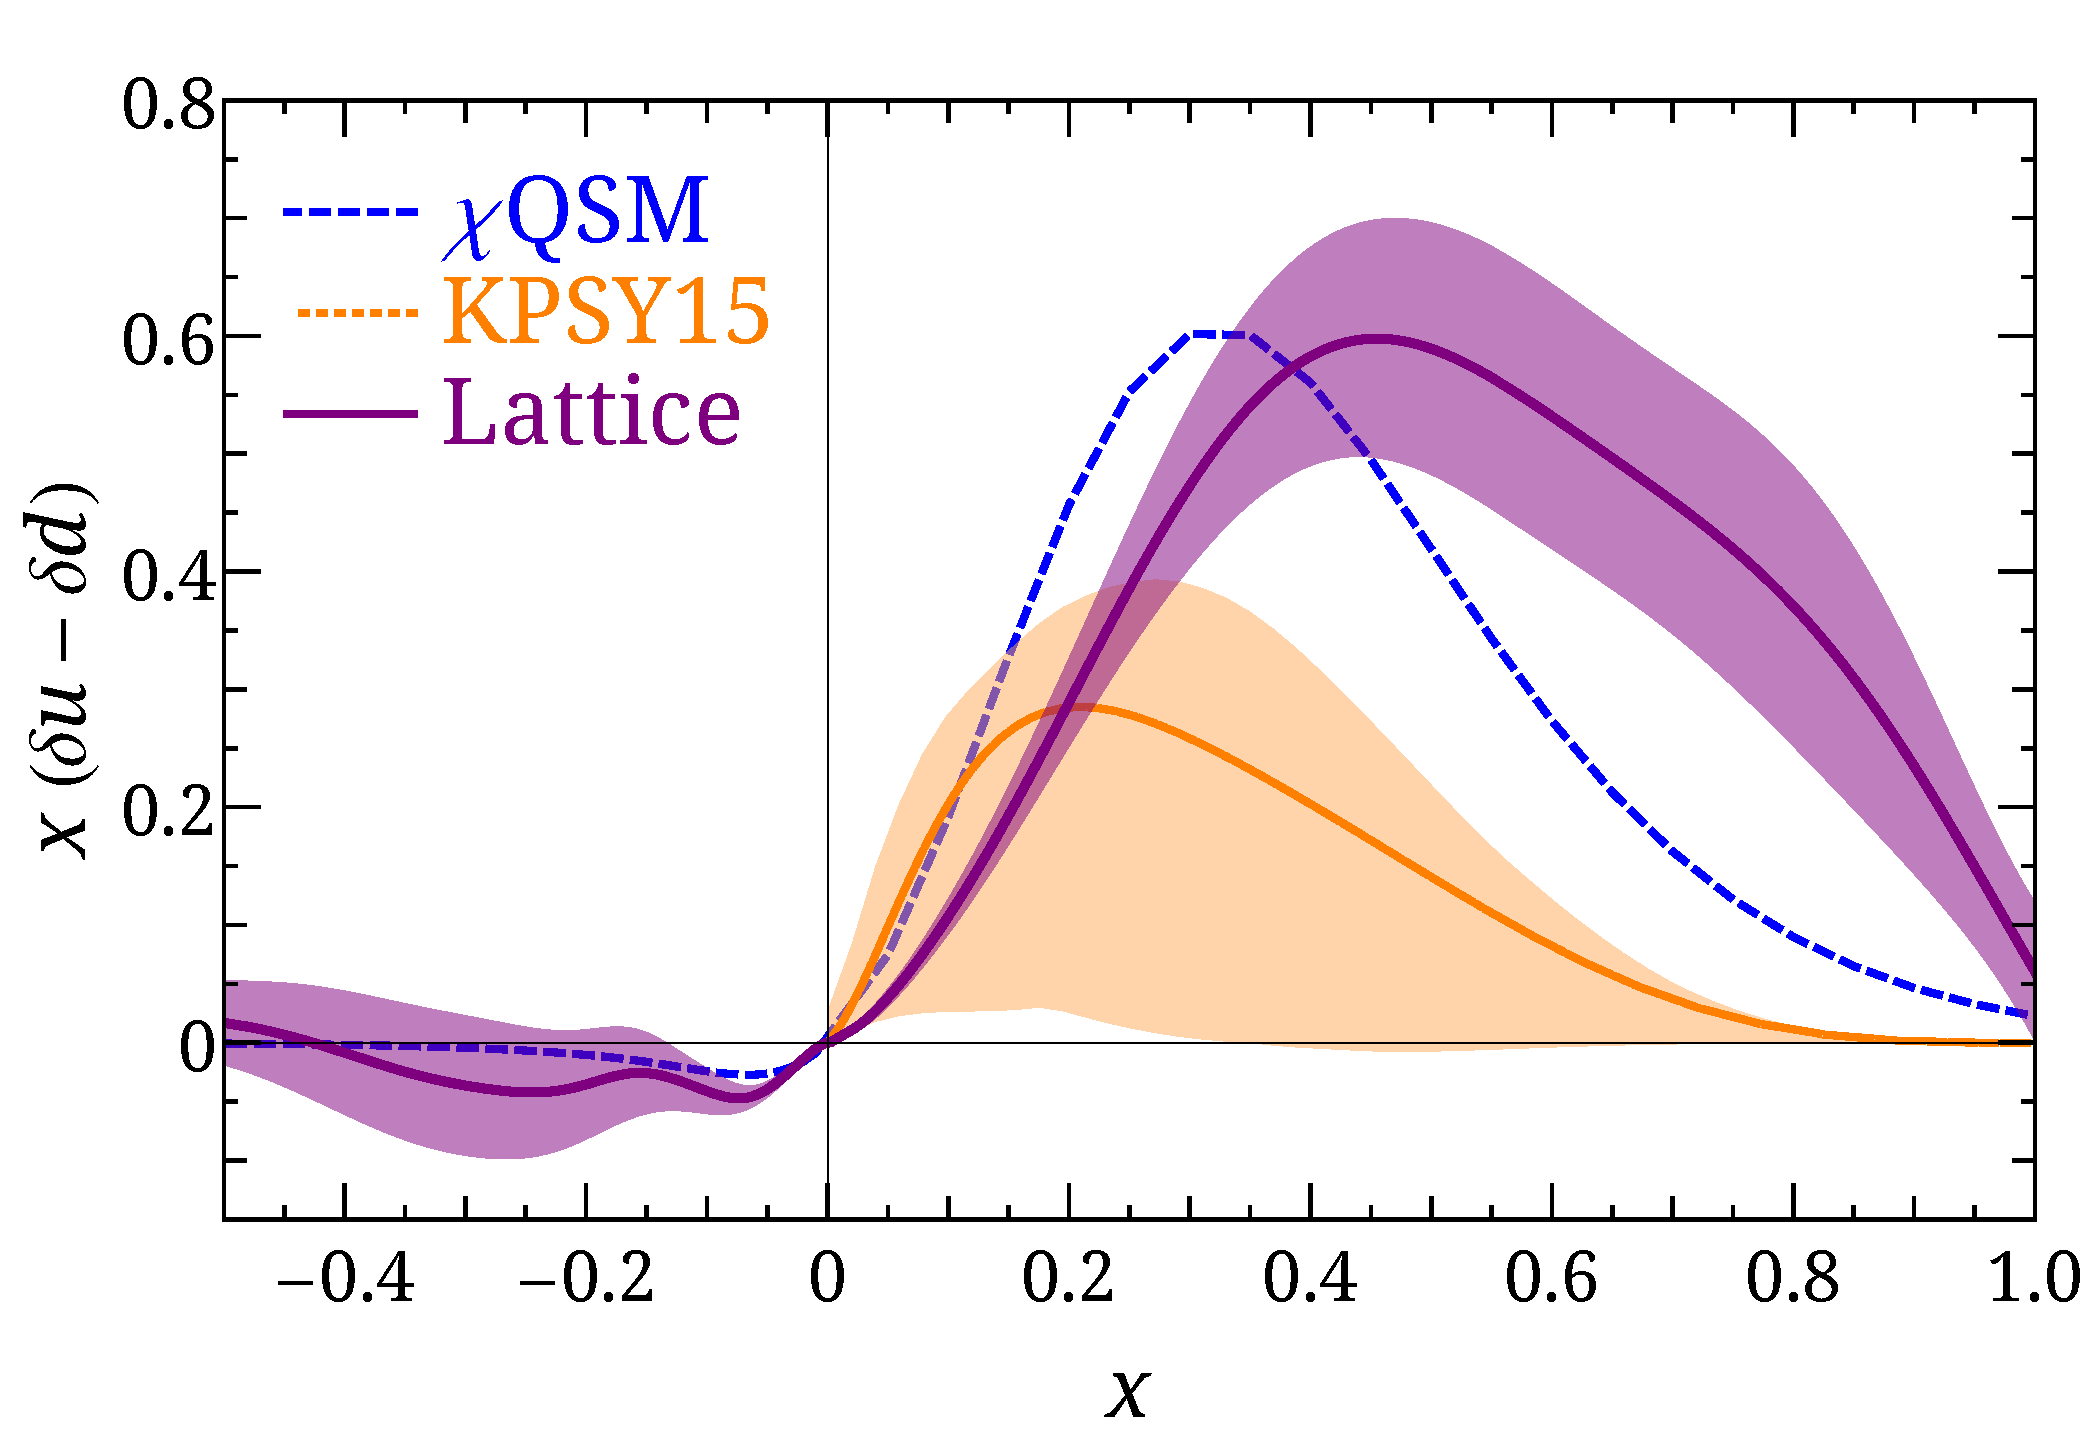
\includegraphics[width=0.47\textwidth]{images/transversityxfinal}
\caption{(left)
The isovector helicity distribution $x (\Delta u(x)-\Delta d(x))$
(purple band) computed on the lattice, along with selected
global polarized analyses by
NNPDFpol1.1~\cite{Nocera:2014gqa},
JAM~\cite{Jimenez-Delgado:2013boa} (green dot-dashed) and
DSSV09~\cite{deFlorian:2009vb} (brown dotted line),
and a model calculation $\chi$QSM~\cite{Schweitzer:2001sr} (blue dashed line).
Note that the uncertainties in the global analyses are omitted here for visibility reasons.
(right)
The isovector transversity distribution $x(\delta u(x)-\delta d(x))$ computed on the lattice in this work,
along with $\chi$QSM~\cite{Schweitzer:2001sr}
(blue dashed line) and latest phenomenological analysis from Ref.~\cite{Kang:2015msa} (labeled as KPSY15, Orange band).
%
The corresponding sea-quark distributions are 
$\Delta \overline{q}(x) = \Delta q(-x)$ 
and
$\delta \overline{q}(x) = -\delta q(-x)$.}
\label{fig:helicity-transversity}
\end{figure*}
